\begin{solution}
The point light source emits light with spherical symmetry, but because of the cylindrical housing what is interpreted is a light ``cone'' instead. This cone intersecting the wall at $x=-D$ is what gives rise to the hyperbola shown.

\begin{center}
    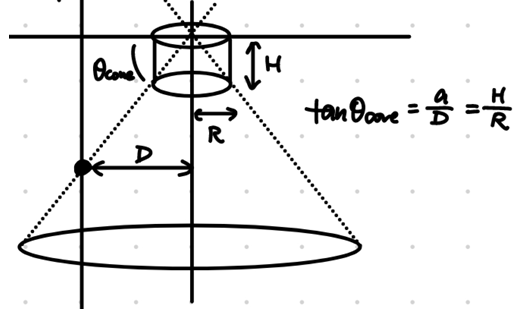
\includegraphics[height=0.35\textwidth]{solutions/figures/lightConeAnswerDiagram.png}
    \hfill
    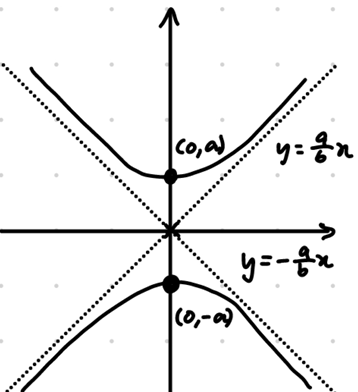
\includegraphics[height=0.35\textwidth]{solutions/figures/lightConeAnswerGraph.png}
\end{center}

By virtue of \href{https://www.youtube.com/watch?v=kfWDkVct5mM}{conic sections} having constant eccentricity, it can be expressed as: $e = \sin\theta_\text{plane}/\sin\theta_\text{cone} = 1/\sin\theta_\text{cone}$ since the wall has $\theta = 90^\circ$. Alternatively, one can also express eccentricity by the formula $e=c/a=\sqrt{a^2+b^2}/a$ where $c=\sqrt{a^2+b^2}$ is the distance from the origin to the focus. Rearranging this gives us:

$$e = \frac{1}{\sin\theta_\text{cone}} = \sqrt{1+\left(\frac{b}{a}\right)^2} \implies \tan\theta_\text{cone} = \frac{a}{b} = 1.33$$

This can then be related to the horizontal distance $D$ by $\tan\theta_\text{cone} = a/D$ to give $D = b = 1.5\text{m}/(4/3) = \boxed{1.125\;\text{m}}$.
\end{solution}